%!TEX root = ULL_thesis_template.tex 
\chapter{Introduction and Background}
\label{intro}
Lorem ipsum dolor sit amet, consectetur adipiscing elit. Vivamus nec tellus eget elit aliquet accumsan sit amet in lacus. In hac habitasse platea dictumst. Ut sit amet elit odio. Aenean lobortis mollis metus, sed consequat neque tristique in. Curabitur nec hendrerit metus. 

\begin{figure}[b!]
\centering
  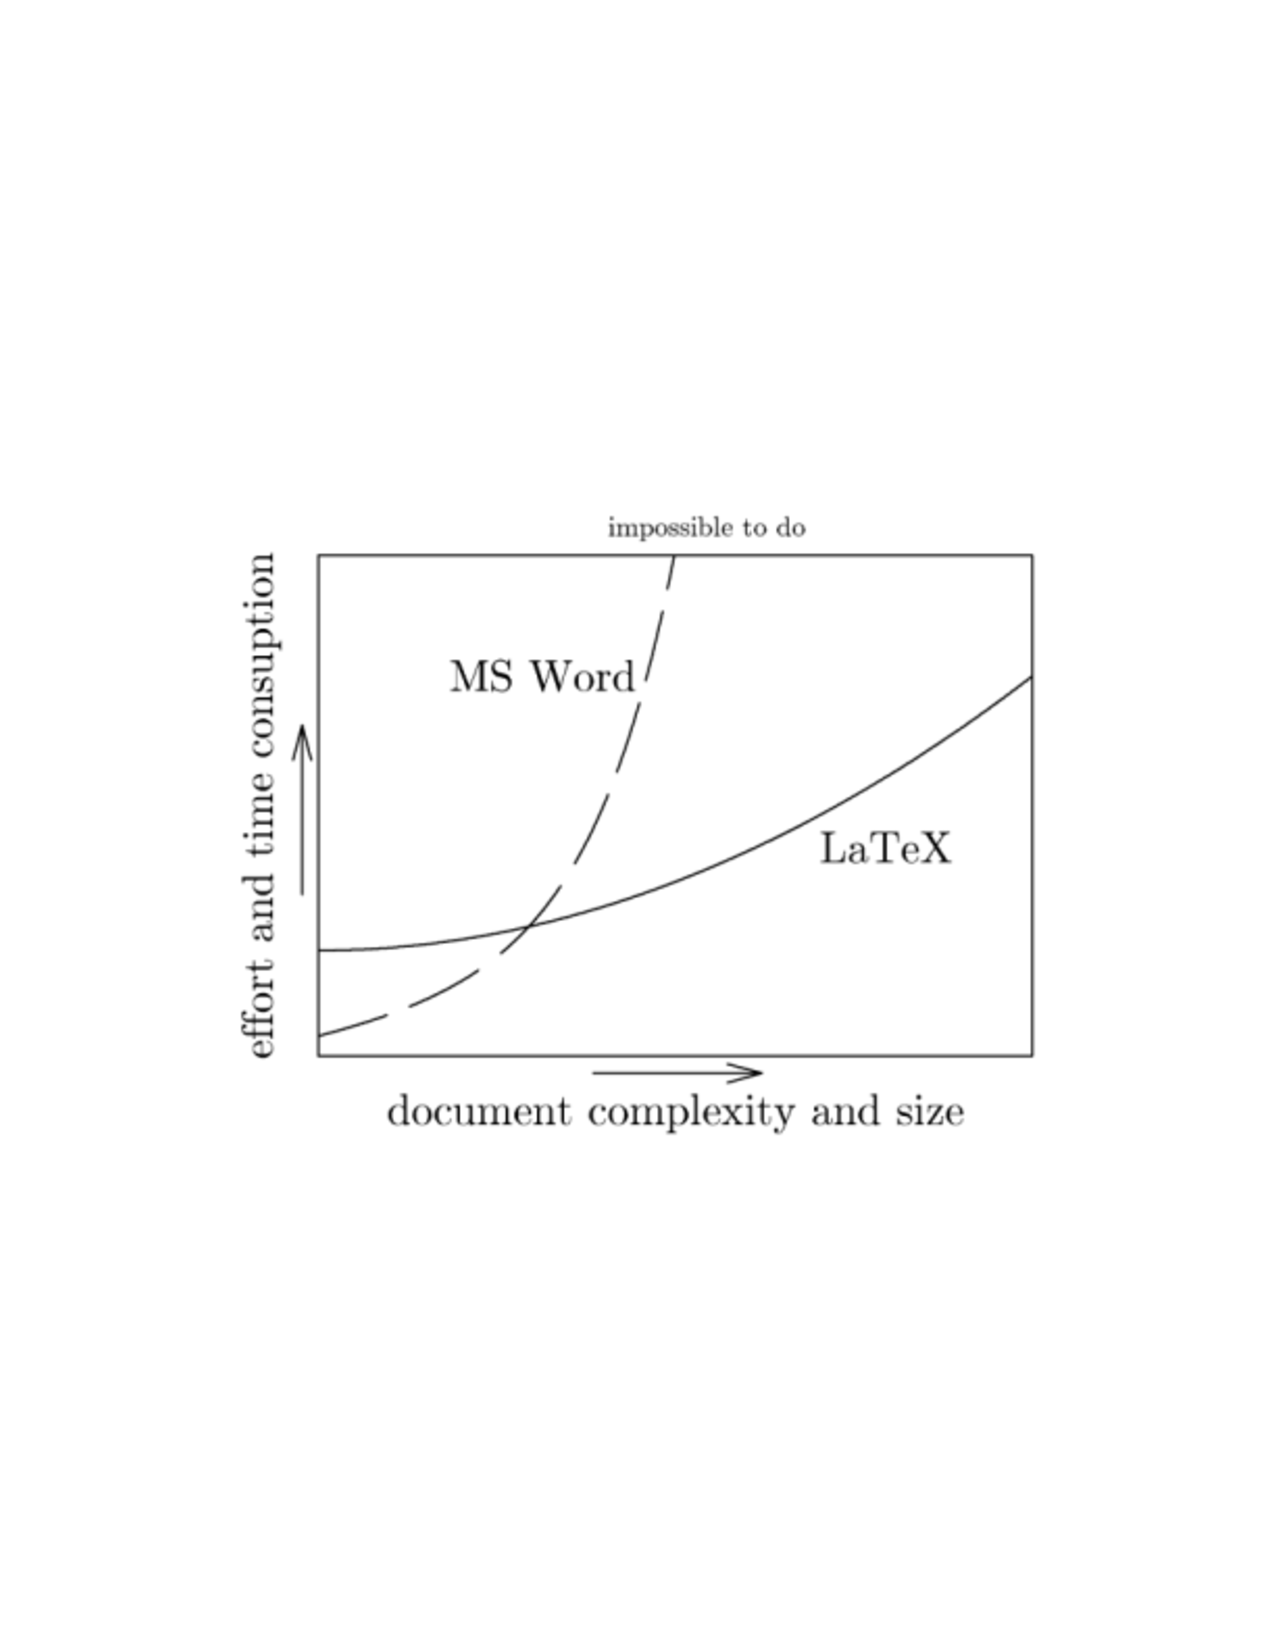
\includegraphics[width=0.5\textwidth]{Figures/Latex.pdf}
  \caption{From Marko Pinteric}
  \label{fig:Latex}
\end{figure}

Praesent non scelerisque urna, vitae iaculis diam. Aliquam nisl est, imperdiet eu nulla sed, bibendum pulvinar arcu. In ultricies purus purus, vulputate congue justo volutpat ut. Donec nunc magna, rutrum nec turpis \ref{fig:Latex} et, viverra efficitur lorem. In hac habitasse platea dictumst. Vestibulum maximus lobortis nisl, eget molestie sem sollicitudin nec. Mauris ut enim eu ipsum auctor rhoncus ac vel eros.

\section{Section}
Vivamus tincidunt, tortor eu rutrum dapibus, orci turpis porta metus, ac iaculis quam eros sollicitudin nisl. Nam id massa elementum, commodo mi at, lobortis nisl. Fusce vestibulum eu lorem non aliquam. Morbi eleifend tortor id metus elementum, ac tincidunt lorem commodo. Pellentesque vestibulum, erat in tempus vehicula, ex urna auctor leo, ut lobortis eros mauris nec erat. Aliquam erat volutpat.

\subsection{Subsection}
Proin vel libero eleifend, convallis nunc eu, sollicitudin elit. Aenean non malesuada ipsum. Vestibulum viverra ullamcorper nibh, vel ornare metus. Nunc quis leo eget ex sollicitudin convallis nec \cite{Maeda1999} eget tortor. In ipsum turpis, pulvinar ut ligula hendrerit, mollis fermentum dui. Mauris augue elit, scelerisque sit amet scelerisque ac, malesuada ac ligula. Vivamus ac ligula ut risus tincidunt hendrerit.

Pellentesque eget accumsan mi. Sed rutrum turpis quis dapibus eleifend. Ut ac ex ullamcorper, pellentesque orci ac, facilisis urna. Phasellus at placerat arcu. Maecenas eu pretium lacus, quis pretium dui. Vestibulum sit amet erat dignissim, suscipit lectus a, malesuada eros. Nullam pellentesque gravida odio, in elementum est bibendum vel. Pellentesque habitant morbi tristique senectus et netus et malesuada fames ac turpis egestas. Mauris in leo rutrum, maximus nisl non, ultricies diam. Donec dictum orci vitae ante efficitur tincidunt id non urna. Lorem ipsum dolor sit amet, consectetur adipiscing elit. Nullam a ipsum ipsum.

\begin{table}[t!]
\centering
\caption{Impulse Amplitudes and Spacing for Two Input Shaper}
\label{table:multi-impulses}
\begin{tabular}{@{}rrrr@{}}
\toprule
\multicolumn{1}{l}{} &  & \multicolumn{2}{c}{Impulse Amplitudes} \\ \midrule
Impulse Times &  & Input $f_1$ & Input $f_2$ \\ \cmidrule(l){3-4} 
0 &  & 0.50 & 0.07 \\
0.84 &  & 0.09 & 0.94 \\
1.69 &  & 0.41 & 0.00 \\ \bottomrule
\end{tabular}
\end{table}